\documentclass[]{article}
\usepackage{lmodern}
\usepackage{amssymb,amsmath}
\usepackage{ifxetex,ifluatex}
\usepackage{fixltx2e} % provides \textsubscript
\ifnum 0\ifxetex 1\fi\ifluatex 1\fi=0 % if pdftex
  \usepackage[T1]{fontenc}
  \usepackage[utf8]{inputenc}
\else % if luatex or xelatex
  \ifxetex
    \usepackage{mathspec}
  \else
    \usepackage{fontspec}
  \fi
  \defaultfontfeatures{Ligatures=TeX,Scale=MatchLowercase}
\fi
% use upquote if available, for straight quotes in verbatim environments
\IfFileExists{upquote.sty}{\usepackage{upquote}}{}
% use microtype if available
\IfFileExists{microtype.sty}{%
\usepackage{microtype}
\UseMicrotypeSet[protrusion]{basicmath} % disable protrusion for tt fonts
}{}
\usepackage[margin=1in]{geometry}
\usepackage{hyperref}
\hypersetup{unicode=true,
            pdftitle={Graficando con R. El inicio},
            pdfauthor={Carlos Iván Espinosa},
            pdfborder={0 0 0},
            breaklinks=true}
\urlstyle{same}  % don't use monospace font for urls
\usepackage{color}
\usepackage{fancyvrb}
\newcommand{\VerbBar}{|}
\newcommand{\VERB}{\Verb[commandchars=\\\{\}]}
\DefineVerbatimEnvironment{Highlighting}{Verbatim}{commandchars=\\\{\}}
% Add ',fontsize=\small' for more characters per line
\usepackage{framed}
\definecolor{shadecolor}{RGB}{248,248,248}
\newenvironment{Shaded}{\begin{snugshade}}{\end{snugshade}}
\newcommand{\KeywordTok}[1]{\textcolor[rgb]{0.13,0.29,0.53}{\textbf{{#1}}}}
\newcommand{\DataTypeTok}[1]{\textcolor[rgb]{0.13,0.29,0.53}{{#1}}}
\newcommand{\DecValTok}[1]{\textcolor[rgb]{0.00,0.00,0.81}{{#1}}}
\newcommand{\BaseNTok}[1]{\textcolor[rgb]{0.00,0.00,0.81}{{#1}}}
\newcommand{\FloatTok}[1]{\textcolor[rgb]{0.00,0.00,0.81}{{#1}}}
\newcommand{\ConstantTok}[1]{\textcolor[rgb]{0.00,0.00,0.00}{{#1}}}
\newcommand{\CharTok}[1]{\textcolor[rgb]{0.31,0.60,0.02}{{#1}}}
\newcommand{\SpecialCharTok}[1]{\textcolor[rgb]{0.00,0.00,0.00}{{#1}}}
\newcommand{\StringTok}[1]{\textcolor[rgb]{0.31,0.60,0.02}{{#1}}}
\newcommand{\VerbatimStringTok}[1]{\textcolor[rgb]{0.31,0.60,0.02}{{#1}}}
\newcommand{\SpecialStringTok}[1]{\textcolor[rgb]{0.31,0.60,0.02}{{#1}}}
\newcommand{\ImportTok}[1]{{#1}}
\newcommand{\CommentTok}[1]{\textcolor[rgb]{0.56,0.35,0.01}{\textit{{#1}}}}
\newcommand{\DocumentationTok}[1]{\textcolor[rgb]{0.56,0.35,0.01}{\textbf{\textit{{#1}}}}}
\newcommand{\AnnotationTok}[1]{\textcolor[rgb]{0.56,0.35,0.01}{\textbf{\textit{{#1}}}}}
\newcommand{\CommentVarTok}[1]{\textcolor[rgb]{0.56,0.35,0.01}{\textbf{\textit{{#1}}}}}
\newcommand{\OtherTok}[1]{\textcolor[rgb]{0.56,0.35,0.01}{{#1}}}
\newcommand{\FunctionTok}[1]{\textcolor[rgb]{0.00,0.00,0.00}{{#1}}}
\newcommand{\VariableTok}[1]{\textcolor[rgb]{0.00,0.00,0.00}{{#1}}}
\newcommand{\ControlFlowTok}[1]{\textcolor[rgb]{0.13,0.29,0.53}{\textbf{{#1}}}}
\newcommand{\OperatorTok}[1]{\textcolor[rgb]{0.81,0.36,0.00}{\textbf{{#1}}}}
\newcommand{\BuiltInTok}[1]{{#1}}
\newcommand{\ExtensionTok}[1]{{#1}}
\newcommand{\PreprocessorTok}[1]{\textcolor[rgb]{0.56,0.35,0.01}{\textit{{#1}}}}
\newcommand{\AttributeTok}[1]{\textcolor[rgb]{0.77,0.63,0.00}{{#1}}}
\newcommand{\RegionMarkerTok}[1]{{#1}}
\newcommand{\InformationTok}[1]{\textcolor[rgb]{0.56,0.35,0.01}{\textbf{\textit{{#1}}}}}
\newcommand{\WarningTok}[1]{\textcolor[rgb]{0.56,0.35,0.01}{\textbf{\textit{{#1}}}}}
\newcommand{\AlertTok}[1]{\textcolor[rgb]{0.94,0.16,0.16}{{#1}}}
\newcommand{\ErrorTok}[1]{\textcolor[rgb]{0.64,0.00,0.00}{\textbf{{#1}}}}
\newcommand{\NormalTok}[1]{{#1}}
\usepackage{graphicx,grffile}
\makeatletter
\def\maxwidth{\ifdim\Gin@nat@width>\linewidth\linewidth\else\Gin@nat@width\fi}
\def\maxheight{\ifdim\Gin@nat@height>\textheight\textheight\else\Gin@nat@height\fi}
\makeatother
% Scale images if necessary, so that they will not overflow the page
% margins by default, and it is still possible to overwrite the defaults
% using explicit options in \includegraphics[width, height, ...]{}
\setkeys{Gin}{width=\maxwidth,height=\maxheight,keepaspectratio}
\IfFileExists{parskip.sty}{%
\usepackage{parskip}
}{% else
\setlength{\parindent}{0pt}
\setlength{\parskip}{6pt plus 2pt minus 1pt}
}
\setlength{\emergencystretch}{3em}  % prevent overfull lines
\providecommand{\tightlist}{%
  \setlength{\itemsep}{0pt}\setlength{\parskip}{0pt}}
\setcounter{secnumdepth}{0}
% Redefines (sub)paragraphs to behave more like sections
\ifx\paragraph\undefined\else
\let\oldparagraph\paragraph
\renewcommand{\paragraph}[1]{\oldparagraph{#1}\mbox{}}
\fi
\ifx\subparagraph\undefined\else
\let\oldsubparagraph\subparagraph
\renewcommand{\subparagraph}[1]{\oldsubparagraph{#1}\mbox{}}
\fi

%%% Use protect on footnotes to avoid problems with footnotes in titles
\let\rmarkdownfootnote\footnote%
\def\footnote{\protect\rmarkdownfootnote}

%%% Change title format to be more compact
\usepackage{titling}

% Create subtitle command for use in maketitle
\newcommand{\subtitle}[1]{
  \posttitle{
    \begin{center}\large#1\end{center}
    }
}

\setlength{\droptitle}{-2em}
  \title{Graficando con R. El inicio}
  \pretitle{\vspace{\droptitle}\centering\huge}
  \posttitle{\par}
  \author{Carlos Iván Espinosa}
  \preauthor{\centering\large\emph}
  \postauthor{\par}
  \predate{\centering\large\emph}
  \postdate{\par}
  \date{Octubre de 2016}


\begin{document}
\maketitle

{
\setcounter{tocdepth}{2}
\tableofcontents
}
\section{Introducción}\label{introduccion}

\begin{center}\rule{0.5\linewidth}{\linethickness}\end{center}

La representación gráfica de los datos es una actividad bastante común,
en todas partes vemos gráficos representando información de todo tipo,
los vemos en textos científicos, divulgativos o en informes de
organismos públicos o privados. Sin embargo, estos no siempre cumplen
con los estándares de una buena gráfica.

El hacer una buena gráfica no es cuestión sencilla y requiere un gran
trabajo de abstracción. En esta lección intentaremos dar algunas pautas
para poder desarrollar gráficas claras y esperamos que bonitas. Claro
como siempre trabajaremos con R.

Pero antes de iniciar con R, es necesario aclaremos algunas cosas
importantes. Intentaremos definir algunos principios básicos e
importantes que deben ser tomados en cuenta para realizar una buena
gráfica, pasaremos luego a entender la anatomía de una gráfica. Con
estos insumos si pasaremos a conocer lo que nos ofrece R para hacer
gráficas.

\subsection{La visualización de datos}\label{la-visualizacion-de-datos}

Nuestros cerebros están mucho más adecuados a captar imágenes más que
números o letras, así que las gráficas es un medio visual para presentar
información. De esta forma debemos pensar que el fin último de un
gráfico es resumir información de tal forma que muestre tendencias y que
permita comparaciones.

Existen muchos principios para realizar una buena gráfica, intentaremos
resumir algunos de ellos.

\begin{itemize}
\item
  Captar la atención del lector. Este posiblemente es uno de los retos
  más grandes cuando estamos haciendo una gráfica, queremos que esta
  llame la atención y el lector se interese por la misma.
\item
  El gráfico debe presentar la información de la forma más sencilla,
  clara y precisa. Por lo tanto debemos asegurarnos que no tenemos
  información de más, si existe algo que borrando no le resta al
  entendimiento del gráfico bórrelo.
\item
  No inducir al error. Esta es una regla que muchos autores coinciden,
  los gráficos tienen el fin de presentar información, por tanto deben
  mostrar lo que esa información dice.
\item
  Los gráficos deben permitir al lector la comparación de datos, mostrar
  tendencias o diferencias entre las variables.
\end{itemize}

Muchas otras reglas han sido discutidas mucho más de lo que uno
realmente piensa, pero creo que lo más importante es entender para que
quiero hacer un gráfico y asegurarme que este esté dando el mensaje que
quiero que dé.

\section{El sistema base de graficas}\label{el-sistema-base-de-graficas}

\begin{center}\rule{0.5\linewidth}{\linethickness}\end{center}

Una de las mayores fortalezas de R es la versatilidad para generar
gráficos de alta calidad, existen muchos paquetes que permiten hacer
gráficos de diferentes características como \texttt{ggplot} o
\texttt{lattice}, sin embargo, ahora nos centraremos en el sistema base.

Antes de empezar, para que se hagan una idea de algunas de las cosas que
podemos hacer con R, permitamos a R que nos dé una muestra de los
gráficos que se pueden hacer.

\begin{Shaded}
\begin{Highlighting}[]
\KeywordTok{demo}\NormalTok{(graphics) }\CommentTok{# Ejecútela usted}
\end{Highlighting}
\end{Shaded}

Sorprendid@, bueno eso no es nada hay muchas cosas que se pueden hacer
con gráficos en R.

\subsection{El lienzo donde graficar}\label{el-lienzo-donde-graficar}

Cuando estamos realizado gráficos en R, al contrario de lo que hemos
visto hasta el momento, R envía el resultado de nuestros códigos a un
dispositivo gráfico (una ventana) y no a un objeto. En el caso de
RStudio es una ventana propia. Esta ventana es como el lienzo donde
dibujaremos el gráfico.

Cuando yo ejecuto un gráfico, por ejemplo con la función \texttt{plot},
la \emph{ventana} (dispositivo gráfico) se abre automáticamente, para
cerrar esta ventana puedo utilizar el comando \texttt{dev.off()}.

La ventana tiene por defecto algunas características que pueden ser
modificadas con la función \texttt{par}. Veamos la ventana que sale por
defecto.

\begin{Shaded}
\begin{Highlighting}[]
\KeywordTok{par}\NormalTok{(}\DataTypeTok{bg=}\StringTok{"grey98"}\NormalTok{)}
\KeywordTok{plot}\NormalTok{(}\DecValTok{1}\NormalTok{:}\DecValTok{100}\NormalTok{, }\DataTypeTok{type=}\StringTok{"n"}\NormalTok{, }\DataTypeTok{axes=}\NormalTok{F, }\DataTypeTok{xlab =} \StringTok{""}\NormalTok{, }\DataTypeTok{ylab=}\StringTok{""}\NormalTok{, }\DataTypeTok{bg=}\StringTok{"white"}\NormalTok{)}
\KeywordTok{rect}\NormalTok{(-}\DecValTok{10}\NormalTok{, -}\DecValTok{10}\NormalTok{, }\DecValTok{120}\NormalTok{, }\DecValTok{120}\NormalTok{, }\DataTypeTok{col=}\StringTok{"white"}\NormalTok{)}
\KeywordTok{box}\NormalTok{(}\DataTypeTok{lty =} \DecValTok{3}\NormalTok{)}
\KeywordTok{mtext}\NormalTok{(}\KeywordTok{c}\NormalTok{(}\StringTok{"side = 1"}\NormalTok{, }\StringTok{"side = 2"}\NormalTok{, }\StringTok{"side = 3"}\NormalTok{, }\StringTok{"side = 4"}\NormalTok{),}
\DataTypeTok{side =} \KeywordTok{c}\NormalTok{(}\DecValTok{1}\NormalTok{, }\DecValTok{2}\NormalTok{, }\DecValTok{3}\NormalTok{, }\DecValTok{4}\NormalTok{), }\DataTypeTok{col =} \StringTok{"grey"}\NormalTok{, }\DataTypeTok{line =} \DecValTok{1}\NormalTok{, }\DataTypeTok{cex =} \FloatTok{1.5}\NormalTok{)}
\end{Highlighting}
\end{Shaded}

\begin{figure}

{\centering 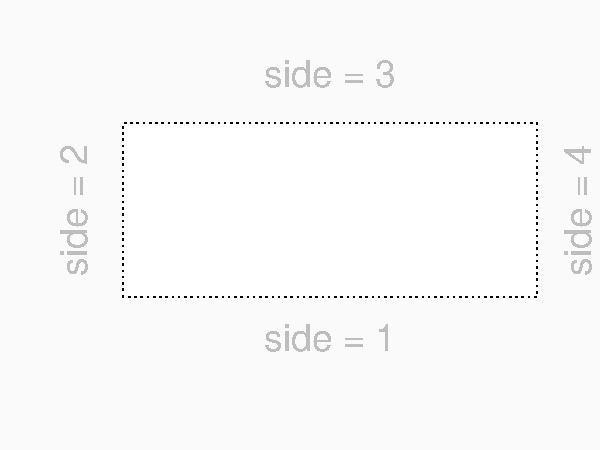
\includegraphics{index_files/figure-latex/unnamed-chunk-2-1} 

}

\caption{Lienzo con características por defecto}\label{fig:unnamed-chunk-2}
\end{figure}

\begin{Shaded}
\begin{Highlighting}[]
\CommentTok{#dev.off()}
\end{Highlighting}
\end{Shaded}

He modificado una característica, el fondo del lienzo, lo normal es que
el lienzo sea de color blanco y yo le he dicho que sea de color
\emph{grey98}. Luego volveremos a este punto.

Como se ve en el gráfico inicialmente podemos ver dos partes distintas,
la región del plot (el cuadrado en blanco), es la zona donde se
dibujaran los datos. El área en gris son los márgenes de cada uno de los
lados (side). Cada lado siempre mantendrá ese orden, el lado uno es el
inferior, el dos el izquierdo, el tres el superior y el cuatro el
derecho. Todos las características de este lienzo pueden ser controladas
desde la función \texttt{par}. Por ejemplo, los márgenes pueden ser
modificados utilizando la función \texttt{mar} dentro de \texttt{par}.
Modifiquemos los márgenes.

\begin{Shaded}
\begin{Highlighting}[]
\KeywordTok{par}\NormalTok{(}\DataTypeTok{bg=}\StringTok{"grey98"}\NormalTok{, }\DataTypeTok{mar=}\KeywordTok{c}\NormalTok{(}\DecValTok{3}\NormalTok{,}\DecValTok{3}\NormalTok{,}\DecValTok{3}\NormalTok{,}\DecValTok{3}\NormalTok{))}
\KeywordTok{plot}\NormalTok{(}\DecValTok{1}\NormalTok{:}\DecValTok{100}\NormalTok{, }\DataTypeTok{type=}\StringTok{"n"}\NormalTok{, }\DataTypeTok{axes=}\NormalTok{F, }\DataTypeTok{xlab =} \StringTok{""}\NormalTok{, }\DataTypeTok{ylab=}\StringTok{""}\NormalTok{, }\DataTypeTok{bg=}\StringTok{"white"}\NormalTok{)}
\KeywordTok{rect}\NormalTok{(-}\DecValTok{10}\NormalTok{, -}\DecValTok{10}\NormalTok{, }\DecValTok{120}\NormalTok{, }\DecValTok{120}\NormalTok{, }\DataTypeTok{col=}\StringTok{"white"}\NormalTok{)}
\KeywordTok{box}\NormalTok{(}\DataTypeTok{lty =} \DecValTok{3}\NormalTok{)}
\KeywordTok{mtext}\NormalTok{(}\KeywordTok{c}\NormalTok{(}\StringTok{"side = 1"}\NormalTok{, }\StringTok{"side = 2"}\NormalTok{, }\StringTok{"side = 3"}\NormalTok{, }\StringTok{"side = 4"}\NormalTok{),}
\DataTypeTok{side =} \KeywordTok{c}\NormalTok{(}\DecValTok{1}\NormalTok{, }\DecValTok{2}\NormalTok{, }\DecValTok{3}\NormalTok{, }\DecValTok{4}\NormalTok{), }\DataTypeTok{col =} \StringTok{"grey"}\NormalTok{, }\DataTypeTok{line =} \DecValTok{1}\NormalTok{, }\DataTypeTok{cex =} \FloatTok{1.5}\NormalTok{)}
\end{Highlighting}
\end{Shaded}

\begin{figure}

{\centering 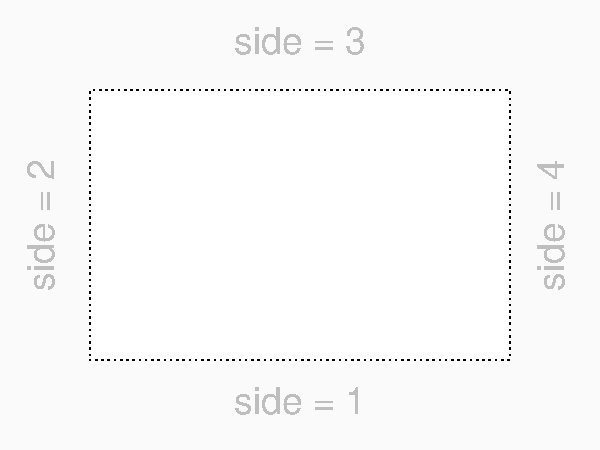
\includegraphics{index_files/figure-latex/unnamed-chunk-3-1} 

}

\caption{Reduciendo los márgenes del lienzo}\label{fig:unnamed-chunk-3}
\end{figure}

Podemos comparar con la anterior figura, ahora vemos que los márgenes se
han hecho más pequeños. la función \texttt{mar} nos permite modificar en
orden los lados 1,2,3,4. Si usted necesita modificar con un valor
diferente cada lado puede hacerlo.

Puede ver todo lo que puede modificar en el lienzo usando la función
\texttt{par}, ejecute en la consola \textbf{?par} y revise las
funciones.

Ahora otra de las cosas que puede ser importante es poder poner en un
mismo lienzo más de un gráfico. ¿Cómo puedo hacer esto?

\subsubsection{Dividiendo el lienzo}\label{dividiendo-el-lienzo}

La función \texttt{mfcol} me permite generar un lienzo con varias partes
iguales, puedo decir cuántas filas y cuantas columnas. Si quiero dos
gráficos uno debajo de otro lo que debo hacer es \texttt{mfcol=c(2,1)}
se especifica primero las filas y luego las columnas. Si quiero en
cambio un grafico a un lado de otro entonces debo poner
\texttt{mfcol=c(1,2)}.

\begin{Shaded}
\begin{Highlighting}[]
\KeywordTok{par}\NormalTok{(}\DataTypeTok{bg=}\StringTok{"grey98"}\NormalTok{, }\DataTypeTok{mar=}\KeywordTok{c}\NormalTok{(}\DecValTok{3}\NormalTok{,}\DecValTok{3}\NormalTok{,}\DecValTok{3}\NormalTok{,}\DecValTok{3}\NormalTok{), }\DataTypeTok{mfcol=}\KeywordTok{c}\NormalTok{(}\DecValTok{1}\NormalTok{,}\DecValTok{2}\NormalTok{))}
\CommentTok{#Primer gráfico}
\KeywordTok{plot}\NormalTok{(}\DecValTok{1}\NormalTok{:}\DecValTok{100}\NormalTok{, }\DataTypeTok{type=}\StringTok{"n"}\NormalTok{, }\DataTypeTok{axes=}\NormalTok{F, }\DataTypeTok{xlab =} \StringTok{""}\NormalTok{, }\DataTypeTok{ylab=}\StringTok{""}\NormalTok{, }\DataTypeTok{bg=}\StringTok{"white"}\NormalTok{)}
\KeywordTok{rect}\NormalTok{(-}\DecValTok{10}\NormalTok{, -}\DecValTok{10}\NormalTok{, }\DecValTok{120}\NormalTok{, }\DecValTok{120}\NormalTok{, }\DataTypeTok{col=}\StringTok{"white"}\NormalTok{)}
\KeywordTok{box}\NormalTok{(}\DataTypeTok{lty =} \DecValTok{3}\NormalTok{)}
\KeywordTok{mtext}\NormalTok{(}\KeywordTok{c}\NormalTok{(}\StringTok{"side = 1"}\NormalTok{, }\StringTok{"side = 2"}\NormalTok{, }\StringTok{"side = 3"}\NormalTok{, }\StringTok{"side = 4"}\NormalTok{),}
\DataTypeTok{side =} \KeywordTok{c}\NormalTok{(}\DecValTok{1}\NormalTok{, }\DecValTok{2}\NormalTok{, }\DecValTok{3}\NormalTok{, }\DecValTok{4}\NormalTok{), }\DataTypeTok{col =} \StringTok{"grey"}\NormalTok{, }\DataTypeTok{line =} \DecValTok{1}\NormalTok{, }\DataTypeTok{cex =} \FloatTok{1.5}\NormalTok{)}
\CommentTok{#Segundo gráfico}
\KeywordTok{plot}\NormalTok{(}\DecValTok{1}\NormalTok{:}\DecValTok{100}\NormalTok{, }\DataTypeTok{type=}\StringTok{"n"}\NormalTok{, }\DataTypeTok{axes=}\NormalTok{F, }\DataTypeTok{xlab =} \StringTok{""}\NormalTok{, }\DataTypeTok{ylab=}\StringTok{""}\NormalTok{, }\DataTypeTok{bg=}\StringTok{"white"}\NormalTok{)}
\KeywordTok{rect}\NormalTok{(-}\DecValTok{10}\NormalTok{, -}\DecValTok{10}\NormalTok{, }\DecValTok{120}\NormalTok{, }\DecValTok{120}\NormalTok{, }\DataTypeTok{col=}\StringTok{"white"}\NormalTok{)}
\KeywordTok{box}\NormalTok{(}\DataTypeTok{lty =} \DecValTok{3}\NormalTok{)}
\KeywordTok{mtext}\NormalTok{(}\KeywordTok{c}\NormalTok{(}\StringTok{"side = 1"}\NormalTok{, }\StringTok{"side = 2"}\NormalTok{, }\StringTok{"side = 3"}\NormalTok{, }\StringTok{"side = 4"}\NormalTok{),}
\DataTypeTok{side =} \KeywordTok{c}\NormalTok{(}\DecValTok{1}\NormalTok{, }\DecValTok{2}\NormalTok{, }\DecValTok{3}\NormalTok{, }\DecValTok{4}\NormalTok{), }\DataTypeTok{col =} \StringTok{"grey"}\NormalTok{, }\DataTypeTok{line =} \DecValTok{1}\NormalTok{, }\DataTypeTok{cex =} \FloatTok{1.5}\NormalTok{)}
\end{Highlighting}
\end{Shaded}

\begin{figure}

{\centering 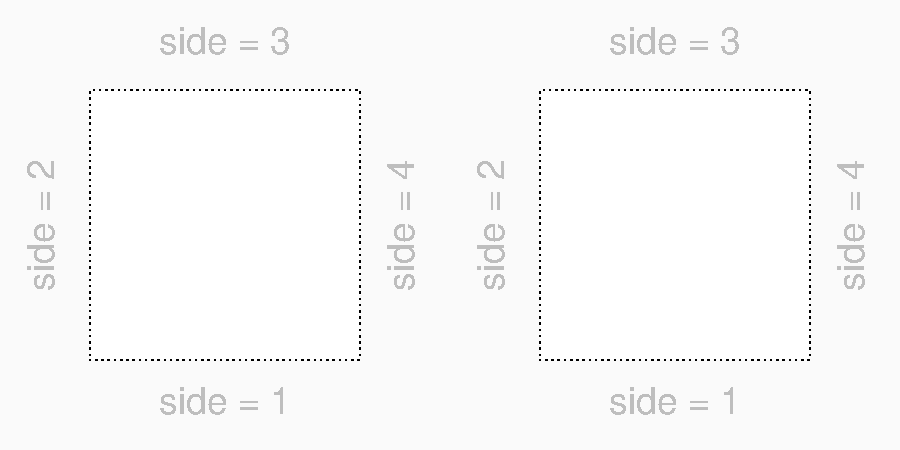
\includegraphics{index_files/figure-latex/unnamed-chunk-4-1} 

}

\caption{Lienzo con dos gráficos de igual tamaño}\label{fig:unnamed-chunk-4}
\end{figure}

La función \texttt{mfcol} es muy usada pero uno de los problemas que
tiene es que todas las particiones tendrán el mismo tamaño, muchas veces
nos interesa que un gráfico sea más grande que otro. Usaremos la función
\texttt{layout} que nos permite partir el lienzo como queramos. El
argumento principal de esta función es una matriz con números enteros
que indican el número de partes que queremos obtener.

\begin{Shaded}
\begin{Highlighting}[]
\KeywordTok{layout}\NormalTok{(}\KeywordTok{matrix}\NormalTok{(}\KeywordTok{c}\NormalTok{(}\DecValTok{1}\NormalTok{,}\DecValTok{2}\NormalTok{,}\DecValTok{3}\NormalTok{,}\DecValTok{3}\NormalTok{), }\DecValTok{2}\NormalTok{, }\DecValTok{2}\NormalTok{))}
\KeywordTok{par}\NormalTok{(}\DataTypeTok{mar=}\KeywordTok{c}\NormalTok{(}\DecValTok{1}\NormalTok{,}\DecValTok{1}\NormalTok{,}\DecValTok{1}\NormalTok{,}\DecValTok{1}\NormalTok{), }\DataTypeTok{bg=}\StringTok{"grey98"}\NormalTok{)}

\CommentTok{#Primer gráfico}
\KeywordTok{plot}\NormalTok{(}\DecValTok{1}\NormalTok{:}\DecValTok{100}\NormalTok{, }\DataTypeTok{type=}\StringTok{"n"}\NormalTok{, }\DataTypeTok{axes=}\NormalTok{F, }\DataTypeTok{xlab =} \StringTok{""}\NormalTok{, }\DataTypeTok{ylab=}\StringTok{""}\NormalTok{, }\DataTypeTok{bg=}\StringTok{"white"}\NormalTok{)}
\KeywordTok{rect}\NormalTok{(-}\DecValTok{10}\NormalTok{, -}\DecValTok{10}\NormalTok{, }\DecValTok{120}\NormalTok{, }\DecValTok{120}\NormalTok{, }\DataTypeTok{col=}\StringTok{"white"}\NormalTok{)}
\KeywordTok{box}\NormalTok{(}\DataTypeTok{lty =} \DecValTok{3}\NormalTok{)}
\CommentTok{#Segundo gráfico}
\KeywordTok{plot}\NormalTok{(}\DecValTok{1}\NormalTok{:}\DecValTok{100}\NormalTok{, }\DataTypeTok{type=}\StringTok{"n"}\NormalTok{, }\DataTypeTok{axes=}\NormalTok{F, }\DataTypeTok{xlab =} \StringTok{""}\NormalTok{, }\DataTypeTok{ylab=}\StringTok{""}\NormalTok{, }\DataTypeTok{bg=}\StringTok{"white"}\NormalTok{)}
\KeywordTok{rect}\NormalTok{(-}\DecValTok{10}\NormalTok{, -}\DecValTok{10}\NormalTok{, }\DecValTok{120}\NormalTok{, }\DecValTok{120}\NormalTok{, }\DataTypeTok{col=}\StringTok{"white"}\NormalTok{)}
\KeywordTok{box}\NormalTok{(}\DataTypeTok{lty =} \DecValTok{3}\NormalTok{)}
\CommentTok{#tercer gráfico}
\KeywordTok{plot}\NormalTok{(}\DecValTok{1}\NormalTok{:}\DecValTok{100}\NormalTok{, }\DataTypeTok{type=}\StringTok{"n"}\NormalTok{, }\DataTypeTok{axes=}\NormalTok{F, }\DataTypeTok{xlab =} \StringTok{""}\NormalTok{, }\DataTypeTok{ylab=}\StringTok{""}\NormalTok{, }\DataTypeTok{bg=}\StringTok{"white"}\NormalTok{)}
\KeywordTok{rect}\NormalTok{(-}\DecValTok{10}\NormalTok{, -}\DecValTok{10}\NormalTok{, }\DecValTok{120}\NormalTok{, }\DecValTok{120}\NormalTok{, }\DataTypeTok{col=}\StringTok{"white"}\NormalTok{)}
\KeywordTok{box}\NormalTok{(}\DataTypeTok{lty =} \DecValTok{3}\NormalTok{)}
\end{Highlighting}
\end{Shaded}

\begin{figure}

{\centering 
\includegraphics{index_files/figure-latex/unnamed-chunk-5-1} 

}

\caption{Lienzo con dos gráficos de tamaño variable}\label{fig:unnamed-chunk-5}
\end{figure}

Si recordamos en lecciones anteriores hemos visto la función matrix, en
esta la primera parte es el vector con los números que se escribirán
dentro de la matriz (en este caso \emph{c(1,2,3,3)}) y la segunda parte
indica las filas y columnas (en este caso 2 filas y 2 columnas). Si
quisiésemos que la gráfica grande este en el lado izquierdo el número 1
debería repetirse (\emph{c(1,1,2,3)}). Inténtalo ahora tú.

Pero qué pasa si queremos por ejemplo hacer los gráficos de diferente
tamaño. Podemos utilizar la misma función pero agregamos los argumentos
\emph{widths} y \emph{heights}, estos argumentos generan cambios
relativos entre las partes, si pongo por ejemplo en widths=c(1,3) los
anchos de las gráficas será la segunda columna 3 veces la primera, de
forma parecida con heights condicionará los altos de las filas.

\begin{Shaded}
\begin{Highlighting}[]
\KeywordTok{layout}\NormalTok{(}\KeywordTok{matrix}\NormalTok{(}\KeywordTok{c}\NormalTok{(}\DecValTok{1}\NormalTok{,}\DecValTok{1}\NormalTok{,}\DecValTok{2}\NormalTok{,}\DecValTok{3}\NormalTok{), }\DecValTok{2}\NormalTok{, }\DecValTok{2}\NormalTok{, }\DataTypeTok{byrow =} \OtherTok{TRUE}\NormalTok{), }
       \DataTypeTok{widths =} \KeywordTok{c}\NormalTok{(}\DecValTok{2}\NormalTok{,}\DecValTok{3}\NormalTok{), }\DataTypeTok{heights =} \KeywordTok{c}\NormalTok{(}\FloatTok{1.5}\NormalTok{,}\DecValTok{3}\NormalTok{))}
\KeywordTok{par}\NormalTok{(}\DataTypeTok{mar=}\KeywordTok{c}\NormalTok{(}\DecValTok{1}\NormalTok{,}\DecValTok{1}\NormalTok{,}\DecValTok{1}\NormalTok{,}\DecValTok{1}\NormalTok{), }\DataTypeTok{oma=}\KeywordTok{c}\NormalTok{(}\DecValTok{3}\NormalTok{,}\DecValTok{3}\NormalTok{,}\DecValTok{1}\NormalTok{,}\DecValTok{1}\NormalTok{), }\DataTypeTok{bg=}\StringTok{"grey98"}\NormalTok{)}

\CommentTok{#Primer gráfico}
\KeywordTok{plot}\NormalTok{(}\DecValTok{1}\NormalTok{:}\DecValTok{100}\NormalTok{, }\DataTypeTok{type=}\StringTok{"n"}\NormalTok{, }\DataTypeTok{axes=}\NormalTok{F, }\DataTypeTok{xlab =} \StringTok{""}\NormalTok{, }\DataTypeTok{ylab=}\StringTok{""}\NormalTok{, }\DataTypeTok{bg=}\StringTok{"white"}\NormalTok{)}
\KeywordTok{rect}\NormalTok{(-}\DecValTok{10}\NormalTok{, -}\DecValTok{10}\NormalTok{, }\DecValTok{120}\NormalTok{, }\DecValTok{120}\NormalTok{, }\DataTypeTok{col=}\StringTok{"white"}\NormalTok{)}
\KeywordTok{box}\NormalTok{(}\DataTypeTok{lty =} \DecValTok{3}\NormalTok{)}
\CommentTok{#Segundo gráfico}
\KeywordTok{plot}\NormalTok{(}\DecValTok{1}\NormalTok{:}\DecValTok{100}\NormalTok{, }\DataTypeTok{type=}\StringTok{"n"}\NormalTok{, }\DataTypeTok{axes=}\NormalTok{F, }\DataTypeTok{xlab =} \StringTok{""}\NormalTok{, }\DataTypeTok{ylab=}\StringTok{""}\NormalTok{, }\DataTypeTok{bg=}\StringTok{"white"}\NormalTok{)}
\KeywordTok{rect}\NormalTok{(-}\DecValTok{10}\NormalTok{, -}\DecValTok{10}\NormalTok{, }\DecValTok{120}\NormalTok{, }\DecValTok{120}\NormalTok{, }\DataTypeTok{col=}\StringTok{"white"}\NormalTok{)}
\KeywordTok{box}\NormalTok{(}\DataTypeTok{lty =} \DecValTok{3}\NormalTok{)}
\CommentTok{#tercer gráfico}
\KeywordTok{plot}\NormalTok{(}\DecValTok{1}\NormalTok{:}\DecValTok{100}\NormalTok{, }\DataTypeTok{type=}\StringTok{"n"}\NormalTok{, }\DataTypeTok{axes=}\NormalTok{F, }\DataTypeTok{xlab =} \StringTok{""}\NormalTok{, }\DataTypeTok{ylab=}\StringTok{""}\NormalTok{, }\DataTypeTok{bg=}\StringTok{"white"}\NormalTok{)}
\KeywordTok{rect}\NormalTok{(-}\DecValTok{10}\NormalTok{, -}\DecValTok{10}\NormalTok{, }\DecValTok{120}\NormalTok{, }\DecValTok{120}\NormalTok{, }\DataTypeTok{col=}\StringTok{"white"}\NormalTok{)}
\KeywordTok{box}\NormalTok{(}\DataTypeTok{lty =} \DecValTok{3}\NormalTok{)}
\end{Highlighting}
\end{Shaded}

\begin{figure}

{\centering 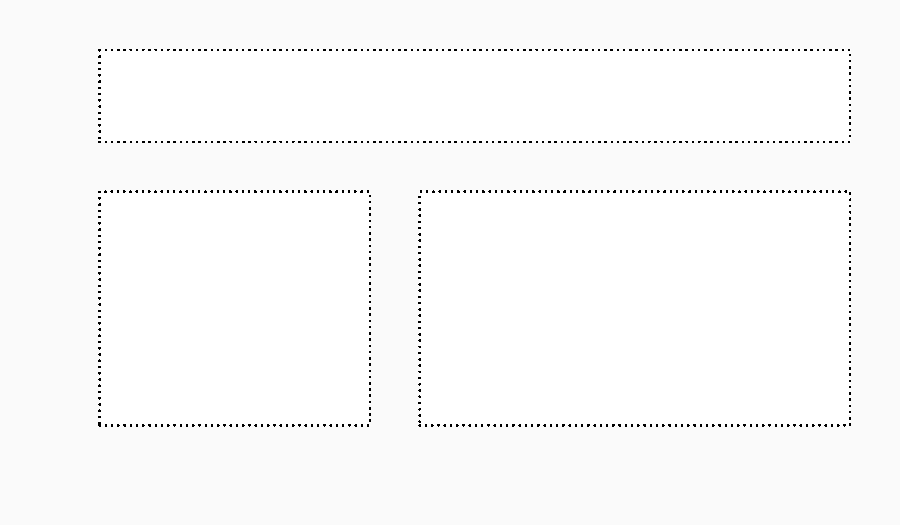
\includegraphics{index_files/figure-latex/unnamed-chunk-6-1} 

}

\caption{Lienzo con dos gráficos de tamaño variable 2}\label{fig:unnamed-chunk-6}
\end{figure}

Como vemos en este caso hemos modificado un poco el lienzo, ahora
tenemos una fila continua en la parte superior y partida en la parte
inferior, para lograr esta partición hemos incluido el argumento
\emph{byrow=T} esto cambia la matriz haciendo que se llene por filas y
no por columnas como sucede por defecto. Además hemos incluido el ancho
y alto de cada fila y columna. Finalmente, en la función \texttt{par}
pusimos el argumento \emph{oma} este argumento permite modificar los
márgenes del grupo de gráficas.

\begin{quote}
Recuerden \textbf{\emph{mar}} modifica los márgenes de cada una de las
gráficas y \textbf{\emph{oma}} el márgen del grupo de gráficas.
\end{quote}

Modifica los márgenes del grupo de gráficas para que comprendas mejor lo
que puede hacer este argumento.

\subsection{Parámetros gráficos}\label{parametros-graficos}

Aunque no lo sabían, ya hemos utilizado algunos parámetros gráficos en
la función \texttt{par}, estos nos han servido para manipular e lienzo.
Usamos \emph{mar} para cambiar márgenes de las gráficas, \emph{oma} para
el conjunto de gráficas, pero además, \emph{bg} para poner un color al
fondo de la gráfica, y \emph{mfcol} para dividir el lienzo en varias
partes iguales.

Vamos a ver unos pocos parámetros más que nos permiten modificar por
ejemplo el tipo de símbolos que graficamos o las líneas, además de los
tamaños de estas dos.

Cuando realizamos un plot según sean nuestros datos, éstos serán
graficados como puntos o como líneas. Podemos darle una forma, un tamaño
y color a estos puntos.

\begin{Shaded}
\begin{Highlighting}[]
\NormalTok{x <-}\StringTok{ }\KeywordTok{rep}\NormalTok{(}\DecValTok{1}\NormalTok{:}\DecValTok{5}\NormalTok{, }\DecValTok{5}\NormalTok{)}
\NormalTok{y <-}\StringTok{ }\KeywordTok{sort}\NormalTok{(}\KeywordTok{rep}\NormalTok{(}\DecValTok{1}\NormalTok{:}\DecValTok{5}\NormalTok{, }\DecValTok{5}\NormalTok{))}
\KeywordTok{par}\NormalTok{(}\DataTypeTok{mar=}\KeywordTok{c}\NormalTok{(}\DecValTok{1}\NormalTok{,}\DecValTok{1}\NormalTok{,}\DecValTok{1}\NormalTok{,}\DecValTok{1}\NormalTok{))}
\KeywordTok{plot}\NormalTok{(x,y, }\DataTypeTok{pch=}\DecValTok{1}\NormalTok{:}\DecValTok{25}\NormalTok{, }\DataTypeTok{col=}\DecValTok{1}\NormalTok{:}\DecValTok{5}\NormalTok{, }\DataTypeTok{cex=}\KeywordTok{seq}\NormalTok{(}\DecValTok{1}\NormalTok{,}\DecValTok{3}\NormalTok{,}\DataTypeTok{length.out =} \DecValTok{25}\NormalTok{), }\DataTypeTok{bg=}\StringTok{"yellow"}\NormalTok{,}
     \DataTypeTok{axes=}\OtherTok{FALSE}\NormalTok{, }\DataTypeTok{xlab=}\StringTok{""}\NormalTok{, }\DataTypeTok{ylab=}\StringTok{""}\NormalTok{, }\DataTypeTok{ylim=}\KeywordTok{c}\NormalTok{(}\DecValTok{0}\NormalTok{,}\DecValTok{6}\NormalTok{))}
\KeywordTok{text}\NormalTok{(x,y}\FloatTok{-0.3}\NormalTok{, }\DataTypeTok{cex=}\FloatTok{0.8}\NormalTok{)}
\end{Highlighting}
\end{Shaded}

\begin{figure}

{\centering 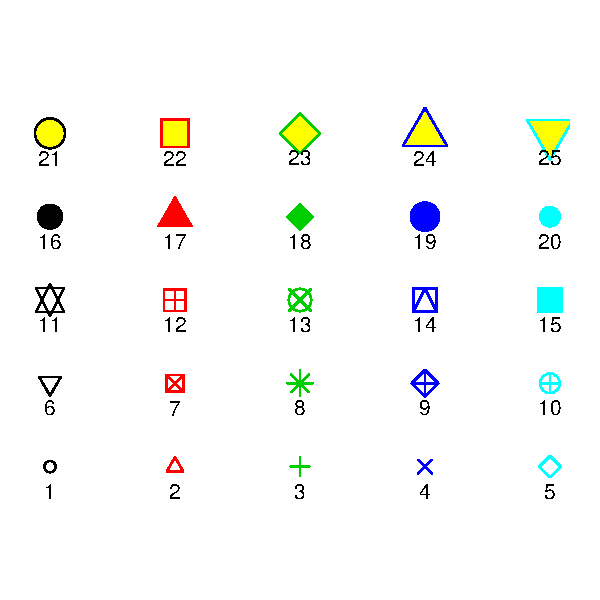
\includegraphics{index_files/figure-latex/unnamed-chunk-7-1} 

}

\caption{Tipos de símbolos gráficos desplegados}\label{fig:unnamed-chunk-7}
\end{figure}

Entendamos lo que hemos hecho. Iremos por cada argumento utilizado,
explicando cual es la función de cada uno de estos. \emph{\textbf{pch}}:
este argumento nos permite modificar el tipo de símbolo gráfico
desplegado, cada número del 1 al 25 corresponde un tipo de símbolo (el
símbolo y su número correspondiente se ve en el gráfico anterior).
\emph{\textbf{col}}: este argumento controla el color que tomará el
símbolo, en nuestro ejemplo hemos escogido los números del 1 al 5 que
corresponden a los colores; negro, rojo, verde, azul y cyan. Podemos
también describir el color que quiero poniendo el nombre en inglés, ej.
``black''. Para ver los colores disponibles digite colors() en la
consola y ejecútelo. \emph{\textbf{cex}}: este argumento controla el
tamaño de los símbolos, por defecto el tamaño es 1, podemos poner
valores menores o superiores. En la figura generamos un vector entre 1 y
3 con 25 particiones, para que los símbolos se desplieguen con tamaños
crecientes entre 1 y 3. \emph{\textbf{bg}}: este argumento controla el
fondo de los símbolos 21 a 25, podemos utilizar cualquier color. Más
adelante conoceremos el resto de argumentos.

También podemos dar formato a las líneas, modificando el tipo de línea y
su tamaño. Veamos cómo podemos hacer esto.

\begin{Shaded}
\begin{Highlighting}[]
\NormalTok{lin <-}\StringTok{ }\KeywordTok{matrix}\NormalTok{(}\KeywordTok{c}\NormalTok{(}\KeywordTok{rep}\NormalTok{(}\DecValTok{1}\NormalTok{,}\DecValTok{5}\NormalTok{), }\KeywordTok{rep}\NormalTok{(}\DecValTok{2}\NormalTok{,}\DecValTok{5}\NormalTok{), }\KeywordTok{rep}\NormalTok{(}\DecValTok{3}\NormalTok{,}\DecValTok{5}\NormalTok{), }\KeywordTok{rep}\NormalTok{(}\DecValTok{4}\NormalTok{,}\DecValTok{5}\NormalTok{), }\KeywordTok{rep}\NormalTok{(}\DecValTok{5}\NormalTok{,}\DecValTok{5}\NormalTok{)), }\DecValTok{5}\NormalTok{,}\DecValTok{5}\NormalTok{) }
\KeywordTok{par}\NormalTok{(}\DataTypeTok{mar=}\KeywordTok{c}\NormalTok{(}\DecValTok{1}\NormalTok{,}\DecValTok{1}\NormalTok{,}\DecValTok{1}\NormalTok{,}\DecValTok{1}\NormalTok{))}
\KeywordTok{matplot}\NormalTok{(lin, }\DataTypeTok{type=}\StringTok{"l"}\NormalTok{, }\DataTypeTok{lty=}\DecValTok{1}\NormalTok{:}\DecValTok{5}\NormalTok{, }\DataTypeTok{lwd=}\KeywordTok{seq}\NormalTok{(}\DecValTok{1}\NormalTok{,}\DecValTok{3}\NormalTok{,}\DataTypeTok{length.out =} \DecValTok{5}\NormalTok{),}
        \DataTypeTok{axes=}\OtherTok{FALSE}\NormalTok{, }\DataTypeTok{ylab=}\StringTok{""}\NormalTok{)}
\end{Highlighting}
\end{Shaded}

\begin{figure}

{\centering 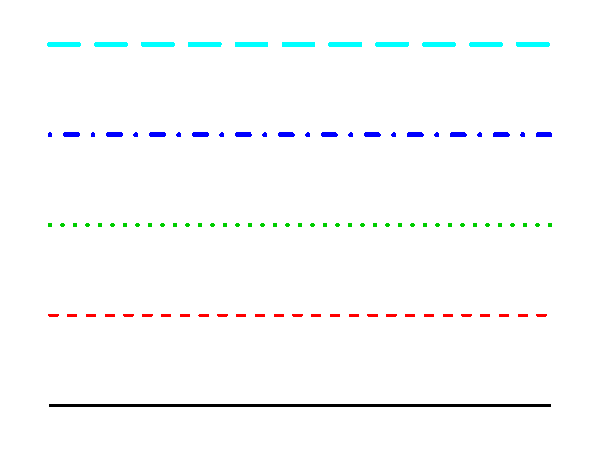
\includegraphics{index_files/figure-latex/unnamed-chunk-8-1} 

}

\caption{Tipos de líneas desplegadas en gráficos}\label{fig:unnamed-chunk-8}
\end{figure}

En este caso el argumento \emph{\textbf{type=``l''}}: define el tipo de
gráfico en este caso le hemos dicho que se dibuje una línea (``l''),
podemos graficar puntos (símbolos) (``p'') o ambos ``b'' o podemos
graficar líneas verticales a cada dato desde el eje central usando
\textbf{type=``h''}. \emph{\textbf{lwd}}: controla el tipo de línea,
continua, entrecortada, puntos, puntos y líneas, etc.
\emph{\textbf{lwd}}: define el tamaño de la línea, por defecto es 1.
Podemos poner un valor para todas o como en el ejemplo un valor para
cada línea.

\subsection{Anatomía de una gráfica}\label{anatomia-de-una-grafica}

Como hemos visto R es muy versátil y podemos hacer una gráfica combinada
que nos presente información complementaria. Ahora pasaremos del lienzo
a la gráfica, pero antes de iniciar los gráficos es necesario conocer
cuáles son las partes de una gráfica.

Utilizaremos datos de R para hacer una gráfica y ver sus partes.

\begin{Shaded}
\begin{Highlighting}[]
\KeywordTok{data}\NormalTok{(cars)}
\KeywordTok{par}\NormalTok{(}\DataTypeTok{mar=}\KeywordTok{c}\NormalTok{(}\DecValTok{4}\NormalTok{,}\DecValTok{3}\NormalTok{,}\DecValTok{3}\NormalTok{,}\DecValTok{4}\NormalTok{), }\DataTypeTok{mgp=}\KeywordTok{c}\NormalTok{(}\FloatTok{1.5}\NormalTok{,}\FloatTok{0.4}\NormalTok{,}\DecValTok{0}\NormalTok{), }\DataTypeTok{tck=}\NormalTok{-}\FloatTok{0.02}\NormalTok{)}

\KeywordTok{plot}\NormalTok{(cars, }\DataTypeTok{xlab=}\StringTok{"Velocidad (mph)"}\NormalTok{, }\DataTypeTok{ylab =} \StringTok{"Distancia"}\NormalTok{, }
     \DataTypeTok{main=}\StringTok{"Relación entre la velocidad de un vehículo}
\StringTok{     y la distancia de frenado"}\NormalTok{, }\DataTypeTok{cex=}\FloatTok{0.8}\NormalTok{, }\DataTypeTok{pch=}\DecValTok{19}\NormalTok{, }\DataTypeTok{cex.main=}\FloatTok{0.9}\NormalTok{, }
     \DataTypeTok{cex.axis=}\FloatTok{0.7}\NormalTok{, }\DataTypeTok{cex.lab=}\FloatTok{0.85}\NormalTok{)}

\KeywordTok{mtext}\NormalTok{(}\StringTok{"Título"}\NormalTok{,}\DataTypeTok{side =} \DecValTok{3}\NormalTok{,}\DataTypeTok{at =} \DecValTok{2}\NormalTok{, }\DataTypeTok{font=}\DecValTok{2}\NormalTok{, }\DataTypeTok{line=}\FloatTok{1.3}\NormalTok{, }\DataTypeTok{cex=}\FloatTok{0.9}\NormalTok{, }\DataTypeTok{col=}\StringTok{"red"}\NormalTok{)}
\KeywordTok{mtext}\NormalTok{(}\StringTok{"Eje x"}\NormalTok{,}\DataTypeTok{side =} \DecValTok{1}\NormalTok{,}\DataTypeTok{at =} \DecValTok{27}\NormalTok{, }\DataTypeTok{font=}\DecValTok{2}\NormalTok{, }\DataTypeTok{line=}\FloatTok{0.4}\NormalTok{, }\DataTypeTok{cex=}\FloatTok{0.8}\NormalTok{, }\DataTypeTok{col=}\StringTok{"blue"}\NormalTok{)}
\KeywordTok{mtext}\NormalTok{(}\StringTok{"Etiqueta del eje x"}\NormalTok{,}\DataTypeTok{side =} \DecValTok{1}\NormalTok{,}\DataTypeTok{at =} \DecValTok{25}\NormalTok{, }\DataTypeTok{font=}\DecValTok{2}\NormalTok{, }\DataTypeTok{line=}\FloatTok{1.5}\NormalTok{, }\DataTypeTok{cex=}\FloatTok{0.8}\NormalTok{, }\DataTypeTok{col=}\StringTok{"red"}\NormalTok{)}
\KeywordTok{mtext}\NormalTok{(}\StringTok{"Eje y"}\NormalTok{,}\DataTypeTok{side =} \DecValTok{1}\NormalTok{,}\DataTypeTok{at =} \DecValTok{2}\NormalTok{, }\DataTypeTok{font=}\DecValTok{2}\NormalTok{, }\DataTypeTok{line=}\FloatTok{0.3}\NormalTok{, }\DataTypeTok{cex=}\FloatTok{0.8}\NormalTok{, }\DataTypeTok{col=}\StringTok{"blue"}\NormalTok{, }\DataTypeTok{las=}\DecValTok{2}\NormalTok{)}
\KeywordTok{mtext}\NormalTok{(}\StringTok{"Etiqueta del eje y"}\NormalTok{,}\DataTypeTok{side =} \DecValTok{1}\NormalTok{,}\DataTypeTok{at =} \FloatTok{0.5}\NormalTok{, }\DataTypeTok{font=}\DecValTok{2}\NormalTok{, }\DataTypeTok{line=}\NormalTok{-}\FloatTok{3.5}\NormalTok{, }\DataTypeTok{cex=}\FloatTok{0.8}\NormalTok{, }\DataTypeTok{col=}\StringTok{"red"}\NormalTok{, }\DataTypeTok{las=}\DecValTok{2}\NormalTok{)}
\KeywordTok{text}\NormalTok{(}\DecValTok{10}\NormalTok{,}\DecValTok{80}\NormalTok{, }\StringTok{"Datos"}\NormalTok{, }\DataTypeTok{col=}\StringTok{"red"}\NormalTok{)}
\end{Highlighting}
\end{Shaded}

\begin{figure}

{\centering 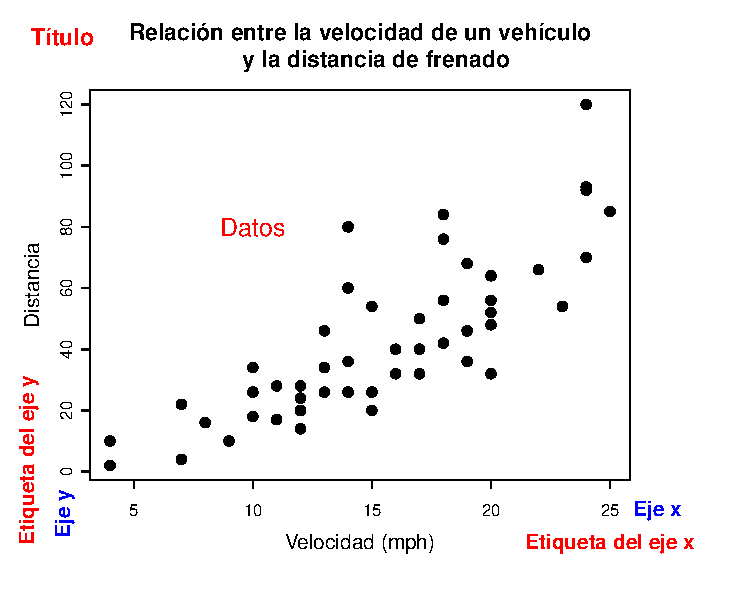
\includegraphics{index_files/figure-latex/unnamed-chunk-9-1} 

}

\caption{Anatomía de un gráfico}\label{fig:unnamed-chunk-9}
\end{figure}

\subsubsection{Los ejes}\label{los-ejes}

Los ejes definen el espacio o rango de una gráfica y lo más común es que
una gráfica tenga dos ejes, los cuales denominamos X e Y. El eje X se
ubica por convenio en la horizontal. En el eje x ponemos las variables
independientes o explicativas, mientras que en el eje y colocamos las
variables de respuesta. En el caso del gráfico anterior la velocidad de
frenado influye en la distancia de frenado de los vehículos.

Cada eje nos permite ver la variación de nuestros datos, vemos que la
velocidad de los vehículos varía entre 3 y 25 mph (parece raro no!, los
datos son de 1920), y la distancia de frenado esta entre 0 y 120
\ldots{}., \emph{se dieron cuenta} hemos encontrado un error en la
etiqueta del gráfico, no sabemos la distancia en que esta medido. Bueno
se los cuento la distancia esta medida en pies. Como podemos ver en el
gráfico R por defecto ajusta los ejes a los datos, siempre es bueno no
tener espacio en blanco, sin embargo, usted podría querer marcar un
límite de los ejes para hacer esto podemos utilizar el argumento
\textbf{xlim} o \textbf{ylim} para modificar el eje x o y
respectivamente. Si quisiéramos incrementar el eje ``Y'' hasta 150
podríamos utilizar el argumento de la siguiente forma:
\textbf{ylim=c(0,150)}.

\subsubsection{Las etiquetas de los
ejes}\label{las-etiquetas-de-los-ejes}

Como nos dimos cuenta hace un momento tener unas etiquetas correctas es
fundamental puesto que estas nos permiten comprender nuestros ejes.
!Cuidado¡ debemos pensarlas bien, ya que tampoco se vale tener unas
etiquetas muy grandes. Recuerda la información debe ser clara y concisa.
La mayor parte de ocasiones las etiquetas de los ejes deben contener la
unidad de medida en la cual se miden las variables.

\begin{quote}
Aprovecho para darte un consejo, siempre es mejor mantener los ejes con
valores pequeños. Si tenemos unos datos en cientos de miles, es mejor
representar los ejes en cientos y en la etiqueta poner el dato en miles.
Veamos un ejemplo: si tengo una etiqueta de ``número de células
cancerígenas'' con unidades del eje entre 1000 y 100000, es mejor
cambiar a una etiqueta ``Miles de células cancerígenas'' con unidades de
entre 1 y 100.
\end{quote}

\subsubsection{El título}\label{el-titulo}

El título es una parte importante del gráfico, al igual que las
etiquetas debemos intentar que el título sea corto y que rescate lo más
importante de la gráfica. Muchas veces se omite el título del gráfico
cuando utilizamos una etiqueta de la figura. Sin embargo, recuerde que
si no tenemos la etiqueta debemos colocar un título.

\subsection{Ejercicio 1}\label{ejercicio-1}

Bueno vamos a parar un poco y ver lo que otra gente ha hecho con
gráficos. Este ejercicio es sencillo y espero divertido.

Piense en una temática específica que le interese, ahora va a buscar 6
gráficos de esa temática, 3 gráficos deben ser buenos gráficos y mire
tres más que usted considere que no son buenos gráficos. Coloque los
gráficos en una hoja de word y describa porque considera que los
gráficos son buenos o malos.

\section{Una gráfica con R}\label{una-grafica-con-r}

\begin{center}\rule{0.5\linewidth}{\linethickness}\end{center}

Vamos mostrar algunas de las funcionalidades de R para hacer gráficos y
dar formato general. Vamos a trabajar con un gráfico bivariado para lo
cual vamos a generar dos series de datos al azar.

El primer paso hacer el gráfico para esto usamos la función
\texttt{plot} y agregamos las dos series de datos que queremos graficar.

\begin{Shaded}
\begin{Highlighting}[]
\KeywordTok{set.seed}\NormalTok{(}\DecValTok{3}\NormalTok{)}
\NormalTok{x <-}\StringTok{ }\KeywordTok{rnorm}\NormalTok{(}\DecValTok{20}\NormalTok{)}
\NormalTok{y <-}\StringTok{ }\KeywordTok{rnorm}\NormalTok{(}\DecValTok{20}\NormalTok{) }

\CommentTok{#Graficamos}
\KeywordTok{plot}\NormalTok{(x,y) }
\end{Highlighting}
\end{Shaded}

\begin{figure}

{\centering 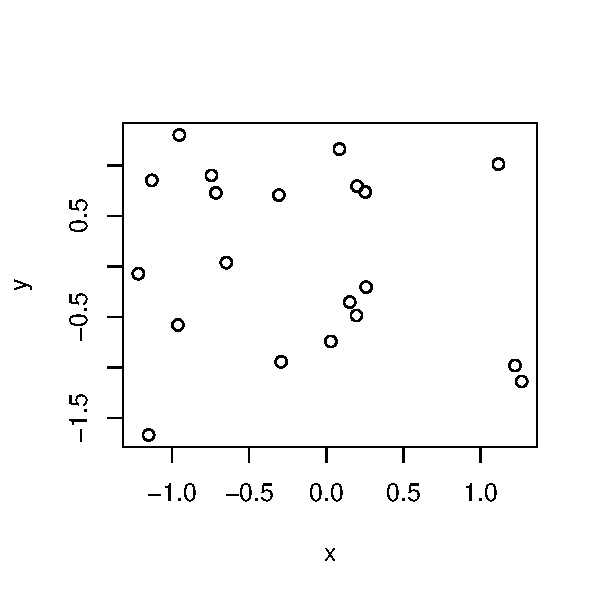
\includegraphics{index_files/figure-latex/unnamed-chunk-10-1} 

}

\caption{Uso de plot, el primer paso}\label{fig:unnamed-chunk-10}
\end{figure}

Como vemos el gráfico por defecto no está del todo mal, ha generado unos
ejes ajustados a los datos, ha dado unas etiquetas a cada eje y puesto
que son datos de dos variables ha elegido puntos para representar los
gráficos. Pero podríamos mejorar la presentación de este gráfico. Por
ahora no hemos hablado de los datos (lo más importante), sino que nos
centraremos en el formato.

Recuerde que hay algunos principios que deberíamos tenerlos presente. Lo
primero es tener un título, y unas etiquetas explicativas para cada eje.
Además vamos a cambiar a unos símbolos que llamen más la atención.

\begin{Shaded}
\begin{Highlighting}[]
\KeywordTok{plot}\NormalTok{(x, y, }\DataTypeTok{xlab=}\StringTok{"números al azar"}\NormalTok{, }\DataTypeTok{ylab=}\StringTok{"números al azar"}\NormalTok{, }\DataTypeTok{pch=}\DecValTok{23}\NormalTok{, }\DataTypeTok{col=}\StringTok{"blue"}\NormalTok{, }\DataTypeTok{bg=}\StringTok{"green"}\NormalTok{, }\DataTypeTok{bty=}\StringTok{"l"}\NormalTok{, }\DataTypeTok{tcl=}\FloatTok{0.4}\NormalTok{, }\DataTypeTok{main=}\StringTok{"Relación entre números al azar"}\NormalTok{, }\DataTypeTok{las=}\DecValTok{1}\NormalTok{, }
     \DataTypeTok{cex=}\FloatTok{1.3}\NormalTok{, }\DataTypeTok{cex.axis=}\FloatTok{0.8}\NormalTok{, }\DataTypeTok{cex.lab=}\FloatTok{0.9}\NormalTok{)}
\end{Highlighting}
\end{Shaded}

\begin{figure}

{\centering 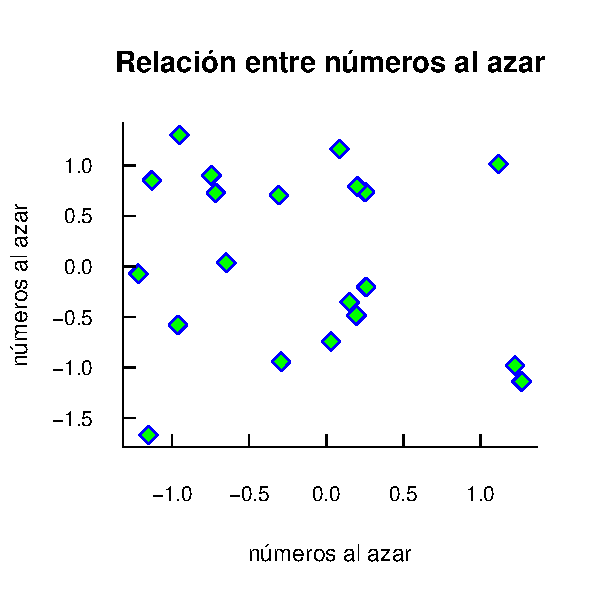
\includegraphics{index_files/figure-latex/unnamed-chunk-11-1} 

}

\caption{Personalizando el grafico en R (1)}\label{fig:unnamed-chunk-11}
\end{figure}

Parece que ha mejorado, pueden intentar cambiando el símbolo utilizado,
seleccionen un símbolo en base de la figura de símbolos. Cambie el
color, utilice \texttt{colors()} para ver que colores hay disponibles.

Que argumentos hemos utilizado. Con \textbf{xlab} y \textbf{ylab}
podemos indicar a R lo que queremos que se escriba como etiqueta del eje
x y el y respectivamente. El argumento \textbf{pch} y \textbf{col} ya
los hemos explicado antes es para cambiar el símbolo y el color. El
argumento \textbf{bty} permite controlar el tipo de caja del área del
gráfico, ``l'' dibuja el primer eje y el segundo eje, nos da como
resultado una L, podría poner ``7'' y se grafican los ejes 3 y 4, ``c''
los ejes 1, 2 y 3. El argumento \textbf{tcl} modifica las marcas de
graduación del gráfico, por defecto es \textbf{-0.5}, nosotros hemos
cambiado a \textbf{0.4} y por eso se han dibujado dentro de la caja. El
argumento \textbf{main} indica el título. \textbf{las} indica la
orientación de los ejes, por defecto es ``las=0'' que indica que el eje
x se escribe horizontalmente y el eje y se escribe verticalmente.
Podemos cambiar a ``las=1'' la opción que elegimos para que el eje ``x''
y ``y'' se escriban horizontalmente. Finalmente, ``las=2'' me permite
poner el eje x verticalmente y el eje y horizontalmente. Como vimos
antes el argumento \textbf{cex} permite controlar el tamaño en general,
en este caso cex solo controla el tamaño del símbolo, ``cex.axis'' y
``cex.lab'' controla el tamaño del eje y el tamaño de la etiqueta del
eje. Podemos utilizar ``cex.main'' para controlar el tamaño del título.

Hemos mejorado pero aún me gustaría modificar algunas otras cosas como
el fondo del lienzo, la distancia a la que se escriben el título y las
etiquetas de los ejes. Vamos a ver cómo cambiar este formato.

\begin{Shaded}
\begin{Highlighting}[]
\KeywordTok{par}\NormalTok{(}\DataTypeTok{bg=}\StringTok{"wheat4"}\NormalTok{, }\DataTypeTok{mar=}\KeywordTok{c}\NormalTok{(}\FloatTok{2.5}\NormalTok{, }\FloatTok{2.5}\NormalTok{,}\DecValTok{3}\NormalTok{, }\FloatTok{0.25}\NormalTok{))}\CommentTok{#cambiamos el fondo y los márgenes}

\KeywordTok{plot}\NormalTok{(x, y, }\DataTypeTok{type=}\StringTok{"n"}\NormalTok{, }\DataTypeTok{xlab=}\StringTok{""}\NormalTok{, }\DataTypeTok{ylab=}\StringTok{""}\NormalTok{, }\DataTypeTok{xlim=}\KeywordTok{c}\NormalTok{(-}\DecValTok{2}\NormalTok{, }\DecValTok{2}\NormalTok{), }
     \DataTypeTok{ylim=}\KeywordTok{c}\NormalTok{(-}\DecValTok{2}\NormalTok{, }\DecValTok{2}\NormalTok{), }\DataTypeTok{xaxt=}\StringTok{"n"}\NormalTok{, }\DataTypeTok{yaxt=}\StringTok{"n"}\NormalTok{) }\CommentTok{#ejecutamos el plot con type="n",}
                                        \CommentTok{#se desplega unicamente la caja (box)}
\KeywordTok{rect}\NormalTok{(-}\DecValTok{3}\NormalTok{, -}\DecValTok{3}\NormalTok{, }\DecValTok{3}\NormalTok{, }\DecValTok{3}\NormalTok{, }\DataTypeTok{col=}\StringTok{"wheat"}\NormalTok{) }\CommentTok{#una caja con de otro color}
\KeywordTok{points}\NormalTok{(x, y, }\DataTypeTok{pch=}\DecValTok{19}\NormalTok{, }\DataTypeTok{col=}\KeywordTok{rgb}\NormalTok{(}\DecValTok{1}\NormalTok{,}\DecValTok{0}\NormalTok{,}\DecValTok{0}\NormalTok{,}\FloatTok{0.6}\NormalTok{), }\DataTypeTok{cex=}\FloatTok{1.5}\NormalTok{) }\CommentTok{#agregamos los puntos}
\KeywordTok{axis}\NormalTok{(}\DataTypeTok{side=}\DecValTok{1}\NormalTok{, }\KeywordTok{c}\NormalTok{(-}\DecValTok{2}\NormalTok{,-}\DecValTok{1}\NormalTok{,}\DecValTok{0}\NormalTok{,}\DecValTok{1}\NormalTok{,}\DecValTok{2}\NormalTok{), }\DataTypeTok{tcl=}\NormalTok{-}\FloatTok{0.4}\NormalTok{, }
     \DataTypeTok{labels=}\OtherTok{FALSE}\NormalTok{, }\DataTypeTok{col=}\StringTok{"white"}\NormalTok{, }\DataTypeTok{lwd=}\DecValTok{2}\NormalTok{) }\CommentTok{#agregamos el primer eje, de color blanco}
\KeywordTok{axis}\NormalTok{(}\DataTypeTok{side=}\DecValTok{2}\NormalTok{, -}\DecValTok{2}\NormalTok{:}\DecValTok{2}\NormalTok{, }\DataTypeTok{tcl=}\NormalTok{-}\FloatTok{0.4}\NormalTok{, }\DataTypeTok{labels=}\OtherTok{FALSE}\NormalTok{, }\DataTypeTok{col=}\StringTok{"white"}\NormalTok{, }\DataTypeTok{lwd=}\DecValTok{2}\NormalTok{) }
\KeywordTok{title}\NormalTok{(}\StringTok{"Relación entre números al azar"}\NormalTok{, }\DataTypeTok{font.main=}\DecValTok{4}\NormalTok{, }\DataTypeTok{adj=}\DecValTok{1}\NormalTok{, }
      \DataTypeTok{cex.main=}\FloatTok{1.2}\NormalTok{, }\DataTypeTok{line=}\FloatTok{1.8}\NormalTok{, }\DataTypeTok{col.main=}\StringTok{"darkred"}\NormalTok{) }\CommentTok{#Agregamos el título}
\KeywordTok{mtext}\NormalTok{(}\StringTok{"números al azar"}\NormalTok{, }\DataTypeTok{side=}\DecValTok{1}\NormalTok{, }\DataTypeTok{line=}\DecValTok{1}\NormalTok{, }\DataTypeTok{at=}\FloatTok{1.5}\NormalTok{, }
      \DataTypeTok{cex=}\FloatTok{0.9}\NormalTok{, }\DataTypeTok{font=}\DecValTok{3}\NormalTok{, }\DataTypeTok{col=}\StringTok{"white"}\NormalTok{)}\CommentTok{#Agregamos etiqueta del eje 1}
\KeywordTok{mtext}\NormalTok{(}\StringTok{"números al azar"}\NormalTok{, }\DataTypeTok{line=}\FloatTok{0.5}\NormalTok{, }\DataTypeTok{at=}\NormalTok{-}\FloatTok{1.8}\NormalTok{, }
      \DataTypeTok{cex=}\FloatTok{0.9}\NormalTok{, }\DataTypeTok{font=}\DecValTok{3}\NormalTok{, }\DataTypeTok{col=}\StringTok{"white"}\NormalTok{)}\CommentTok{#Agregamos etiqueta del eje 2 }
\KeywordTok{mtext}\NormalTok{(-}\DecValTok{2}\NormalTok{:}\DecValTok{2}\NormalTok{, }\DataTypeTok{side=}\DecValTok{1}\NormalTok{, }\DataTypeTok{las=}\DecValTok{1}\NormalTok{, }\DataTypeTok{at=}\NormalTok{-}\DecValTok{2}\NormalTok{:}\DecValTok{2}\NormalTok{, }\DataTypeTok{line=}\FloatTok{0.3}\NormalTok{, }
      \DataTypeTok{col=}\StringTok{"white"}\NormalTok{, }\DataTypeTok{cex=}\FloatTok{0.9}\NormalTok{, }\DataTypeTok{font=}\DecValTok{2}\NormalTok{) }\CommentTok{#Incluimos las leyendas del eje 1}
\KeywordTok{mtext}\NormalTok{(-}\DecValTok{2}\NormalTok{:}\DecValTok{2}\NormalTok{, }\DataTypeTok{side=}\DecValTok{2}\NormalTok{, }\DataTypeTok{las=}\DecValTok{1}\NormalTok{, }\DataTypeTok{at=}\NormalTok{-}\DecValTok{2}\NormalTok{:}\DecValTok{2}\NormalTok{, }\DataTypeTok{line=}\FloatTok{0.5}\NormalTok{,}
      \DataTypeTok{col=}\StringTok{"white"}\NormalTok{, }\DataTypeTok{cex=}\FloatTok{0.9}\NormalTok{, }\DataTypeTok{font=}\DecValTok{2}\NormalTok{) }\CommentTok{#Incluimos las leyendas del eje 2}
\end{Highlighting}
\end{Shaded}

\begin{figure}

{\centering 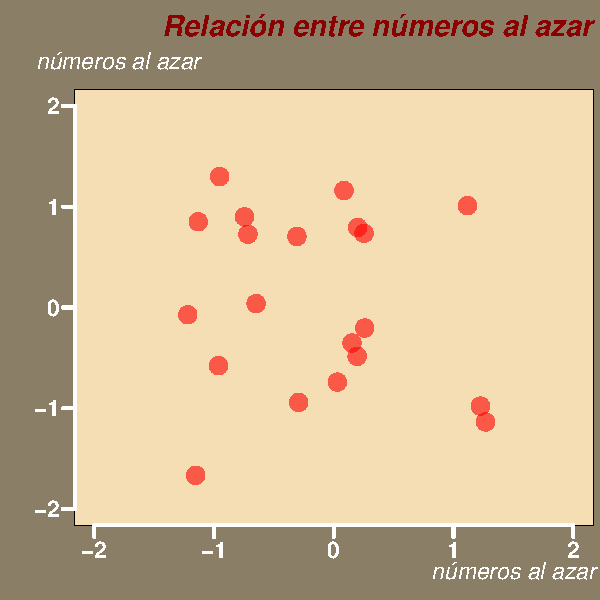
\includegraphics{index_files/figure-latex/unnamed-chunk-12-1} 

}

\caption{Personalizando el grafico en R (2)}\label{fig:unnamed-chunk-12}
\end{figure}

Intentaré explicar rápidamente lo que hemos hecho. - Lo primero es que
graficamos con argumentos de tipo (type) y ejes (xaxt, yaxt) nulo
(``n''), por lo que no se dibujan ni ejes ni puntos. Además, las
etiquetas de los ejes sin datos (xlab=``'', ylab=``'') por lo que R no
escribe etiquetas.

\begin{itemize}
\item
  Con la función \texttt{rect} graficamos un cuadrado mayor al límite
  del gráfico de -3 a 3 y le ponemos un color distinto al fondo.
\item
  Con la función \texttt{points} agregamos los datos con unos símbolos
  determinados y les ponemos un color. Usamos la función \texttt{rgb}
  que nos permite dar un color y hacerlo semitransparente.
\item
  Con la función \texttt{axis} incluimos el eje 1 y 2 (side=1 o 2), le
  damos un vector que usará para poner las marcas, el tamaño de las
  marcas lo controlamos con tcl (tcl=-0.4). Le damos color (col), le
  decimos que no incluya las leyendas (labels=FALSE) y controlamos el
  ancho de la línea del eje (lwd=2).
\item
  Con la función \texttt{title} podemos incluir el título y controlar
  algunos parámetros. El argumento ``font.main'' permite modificar el
  texto con cursivas y negritas como en el gráfico (font.main=4),
  cursivas (font.main=2), negritas (font.main=2) o sin cursivas y sin
  negritas (font.main=4). El argumento adj=1 justifica el texto a la
  derecha, podemos cambiarlo al centro con adj=0.5, o a la izquierda con
  adj=0. El argumento line=1.8 permite alejar o acercar el título del
  gráfico.
\end{itemize}

Me parece que quedo muy bien el gráfico que opinan ustedes?. Lo podrían
hacer mejor, estoy seguro de que si, inténtalo.

\subsection{Ejercicio 2}\label{ejercicio-2}

Modifica los argumentos de esta gráfica, cambia los colores los símbolos
y todo lo que quieras. Intenta hacer un gráfico que se acople a lo que
necesitas y te gusta.

\section{Gráficos de una variable}\label{graficos-de-una-variable}

Bueno creo que hemos logrado hacer cosas interesantes pero solo hemos
jugado, como les decía lo más importante en un gráfico son los datos.
Hasta ahora no nos habíamos preocupado de ello, pero es hora de hacerlo.

\begin{Shaded}
\begin{Highlighting}[]
\KeywordTok{library}\NormalTok{(readxl)}
\NormalTok{ame <-}\StringTok{ }\KeywordTok{read_excel}\NormalTok{(}\StringTok{"AMEBIASIS_LOJA.xlsx"}\NormalTok{,}\DataTypeTok{sheet =} \DecValTok{1}\NormalTok{, }\DataTypeTok{na =} \StringTok{"NA"}\NormalTok{)}\CommentTok{#cargamos los datos}
\NormalTok{pr.edad <-}\StringTok{ }\KeywordTok{tapply}\NormalTok{(ame$}\StringTok{`}\DataTypeTok{Edad en años}\StringTok{`}\NormalTok{, ame$Parroquia, mean)}
                                      \CommentTok{# obtenemos la media de edad por parroquia }
\end{Highlighting}
\end{Shaded}

Una vez que tenemos los datos de la media de edad con amebiasis es
posible que nos interese ver los datos en una gráfica.

\begin{Shaded}
\begin{Highlighting}[]
\KeywordTok{plot}\NormalTok{(pr.edad, }\DataTypeTok{ylab=}\StringTok{"Edad Promedio"}\NormalTok{, }\DataTypeTok{xaxt=}\StringTok{"n"}\NormalTok{, }\DataTypeTok{xlab=}\StringTok{""}\NormalTok{, }\DataTypeTok{pch=}\DecValTok{19}\NormalTok{)}
\end{Highlighting}
\end{Shaded}

\begin{figure}

{\centering 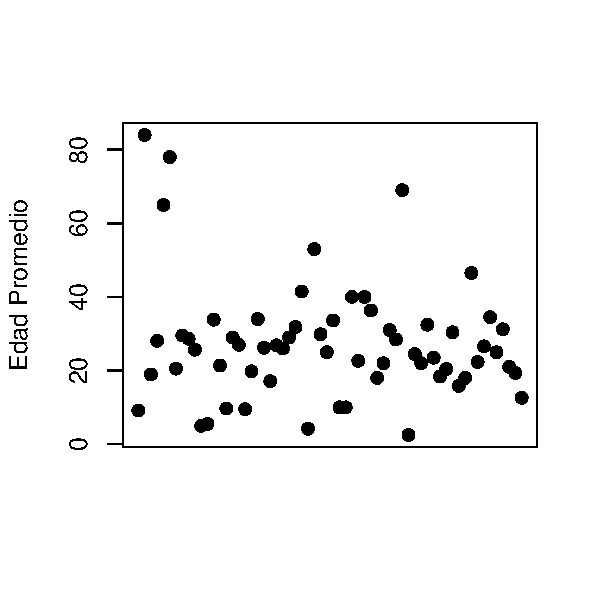
\includegraphics{index_files/figure-latex/unnamed-chunk-14-1} 

}

\caption{Ejemplo de gráfico con una sola variable}\label{fig:unnamed-chunk-14}
\end{figure}

Le hemos pedido que no grafique el eje x, ya que realmente el eje x no
es ninguna variable, lo que estamos graficando es una sola variable, por
lo que lo lógico es que este eje no se grafique. Esta gráfica nos
permite ver la dispersión de los datos, ya podemos ver que la edad más
recurrente en la que se enferman de amebiasis es entre 20 y 30 años. Sin
embargo, una gráfica mejor para resumir una sola variable cuantitativa
como la media de edad sería un diagrama de caja, también conocido como
diagrama de caja y bigote, o boxplot en inglés.

\begin{Shaded}
\begin{Highlighting}[]
\KeywordTok{boxplot}\NormalTok{(pr.edad)}
\end{Highlighting}
\end{Shaded}

\begin{figure}

{\centering 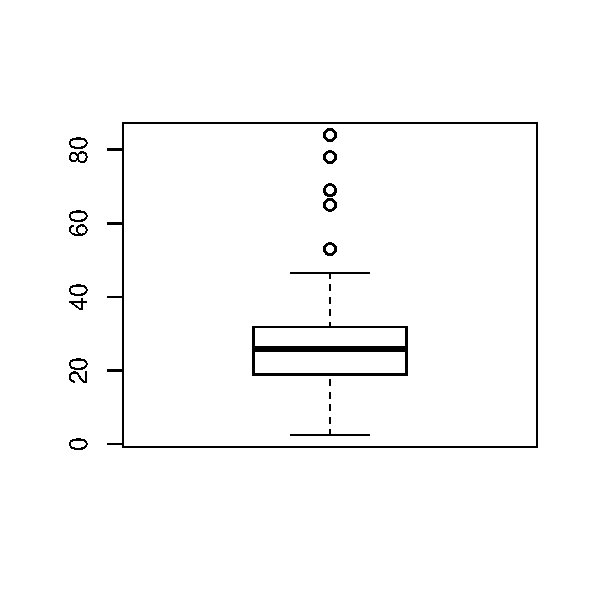
\includegraphics{index_files/figure-latex/unnamed-chunk-15-1} 

}

\caption{Ejemplo de boxplot con una sola variable (1)}\label{fig:unnamed-chunk-15}
\end{figure}

Ahora es mucho más claro que la mediana de nuestros datos están en torno
a los 30 años. Además vemos que algunas parroquias muestran valores
raros superiores a los 50 años. Una buena forma de presentar esta
información es mezclar este boxplot con los datos brutos. Veamos lo que
podemos hacer.

\begin{Shaded}
\begin{Highlighting}[]
\KeywordTok{boxplot}\NormalTok{(pr.edad)}
\KeywordTok{stripchart}\NormalTok{(pr.edad, }\DataTypeTok{method =} \StringTok{"jitter"}\NormalTok{, }\DataTypeTok{jitter =} \FloatTok{0.1}\NormalTok{, }\DataTypeTok{add =}
\OtherTok{TRUE}\NormalTok{, }\DataTypeTok{vertical =} \OtherTok{TRUE}\NormalTok{, }\DataTypeTok{pch=}\DecValTok{19}\NormalTok{)}
\end{Highlighting}
\end{Shaded}

\begin{figure}

{\centering 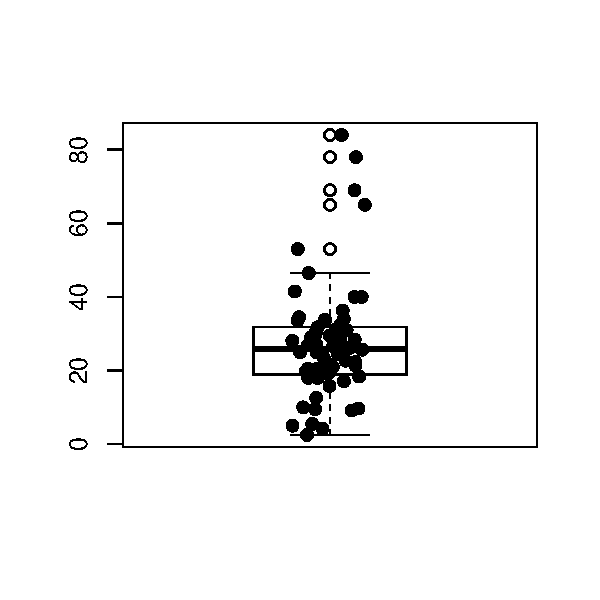
\includegraphics{index_files/figure-latex/unnamed-chunk-16-1} 

}

\caption{Ejemplo de boxplot con una sola variable (1)}\label{fig:unnamed-chunk-16}
\end{figure}

Bueno que les parece, ¿bonito no? Aunque hay muchos elementos que
incluir aún para que esto pueda llamarse gráfico de verdad.

Otra interesante opción es realizar un histograma con esta variable. El
histograma nos muestra la frecuencia de los datos a lo largo de rangos
equitativos de la variable. Al igual que el boxplot nos ayuda ver la
distribución de los datos.

\begin{Shaded}
\begin{Highlighting}[]
\KeywordTok{hist}\NormalTok{(pr.edad)}
\end{Highlighting}
\end{Shaded}

\begin{figure}

{\centering 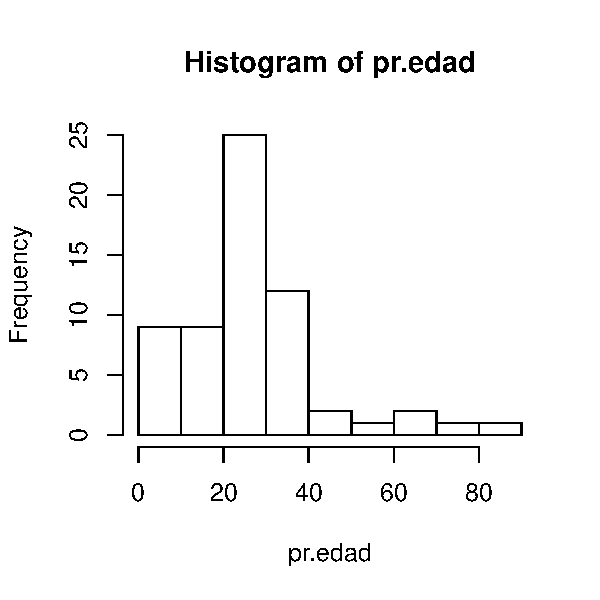
\includegraphics{index_files/figure-latex/unnamed-chunk-17-1} 

}

\caption{Ejemplo de histograma}\label{fig:unnamed-chunk-17}
\end{figure}

\subsection{Ejercicio 3}\label{ejercicio-3}

Nos interesa describir la distribución de edad de las personas que han
padecido Amebiasis.

Incluya los elementos que considere necesarios y póngale el formato de
color y ejes que le parezca al boxplot y al histograma del promedio de
edad por parroquia de las personas con amebiasis. Debe partir el lienzo
en dos partes, podrían ser desiguales para poner en el mismo lienzo las
dos gráficas. Espero tener un gráfico para enmarcar, seguro lo podrá
hacer.


\end{document}
